%!TEX TS-program = pdflatex
\documentclass[10pt,%
	wide,%
	xcolor={x11names},%
	hyperref={colorlinks},%
	pantone312,%
	handout,%
	]{beamer}
%!TEX root = vortrag.tex
% Basics und Codierung
% ===========================================================
\usepackage{wwustyle2}
\usepackage[ngerman]{babel}
\usepackage[utf8]{inputenc}
\usepackage[T1]{fontenc}
\usepackage[german=quotes]{csquotes}
\usepackage{scrtime}
\usepackage{etex}
\usepackage{shellesc}
% ===========================================================

% Fonts und Typographie
% ===========================================================
\usepackage{sourcecodepro}
\usepackage[default]{sourcesanspro}
\usepackage{nimbusmononarrow}
\usepackage{ellipsis}
\newcommand{\bet}[1]{\textbf{\color{maincolor}#1}}
\newcommand{\minor}[1]{\textcolor{black!50}{#1}}
\newcommand{\minoritem}{\item[{\footnotesize \textcolor{black!50}{$\blacktriangleright$}}]}
\newcommand{\code}[1]{\texttt{#1}}
\usepackage{xspace}
\makeatletter 
\xspaceaddexceptions{\grqq \grq \csq@qclose@i \} } 
\makeatother
\usefonttheme[onlymath]{serif}
\usepackage{multicol}
\newcommand{\hyper}[1]{\bet{\underline{\smash{#1}}}}
% ===========================================================

% Farben	
% ===========================================================
	\usepackage{xcolor}
	\definecolor{fbblau}{HTML}{3078AB}
	\definecolor{mediumgray}{gray}{.65}
	\definecolor{blackberry}{rgb}{0.53, 0.0, 0.25}
% ===========================================================

% Mathe-Pakete
% ===========================================================
	\usepackage{mathtools}
	\usepackage{amssymb}
	\usepackage[bigdelims]{newtxmath}

	% Abkürzungen
% ===========================================================
	\newcommand{\BB}{\mathbb{B}}
	\newcommand{\CC}{\mathbb{C}}
	\newcommand{\EE}{\mathbb{E}}
	\newcommand{\FF}{\mathbb{F}}
	\newcommand{\HH}{\mathcal{H}}
	\newcommand{\KK}{\mathbb{K}}
	\newcommand{\LL}{\mathbb{L}}
	\newcommand{\NN}{\mathbb{N}}
	\newcommand{\QQ}{\mathbb{Q}}
	\newcommand{\RR}{\mathbb{R}}
	\newcommand{\ZZ}{\mathbb{Z}}
	\newcommand{\oh}{\mathcal{O}}				% Landau-O
	\newcommand{\ind}{1\hspace{-0,8ex}1} 		% Indikatorfunktion (Doppeleins)
	\newcommand{\bewrueck}{\enquote{$\Leftarrow$}:} 	% Beweis Rückrichtung
	\newcommand{\bewhin}{\enquote{$\Rightarrow$}:}		% Beweis Hinrichtung
	\newcommand{\ol}[1]{\overline{#1}}
	\newcommand{\wt}[1]{\widetilde{#1}}
	\newcommand{\wh}[1]{\widehat{#1}}
% ===========================================================

% Operatoren
% ===========================================================
	\DeclareMathOperator{\id}{id} 				% Identität
	\DeclareMathOperator{\im}{im} 				% image
	\DeclareMathOperator{\pot}{\mathcal{P}}		% Potenzmenge
	\DeclareMathOperator{\sgn}{sgn} 			% Signum
	\DeclareMathOperator{\Sym}{Sym} 			% Symmetrische Gruppe
% ===========================================================

% Klammerungen und ähnliches
% ===========================================================
	\DeclarePairedDelimiter{\absolut}{\lvert}{\rvert}		% Betrag
	\DeclarePairedDelimiter{\ceiling}{\lceil}{\rceil}		% aufrunden
	\DeclarePairedDelimiter{\Floor}{\lfloor}{\rfloor}		% aufrunden
	\DeclarePairedDelimiter{\Norm}{\lVert}{\rVert}			% Norm
	\DeclarePairedDelimiter{\sprod}{\langle}{\rangle}		% spitze Klammern
	\DeclarePairedDelimiter{\enbrace}{(}{)}					% runde Klammern
	\DeclarePairedDelimiter{\benbrace}{\lbrack}{\rbrack}	% eckige Klammern
	\DeclarePairedDelimiter{\penbrace}{\{}{\}}				% geschweifte Klammern
	\newcommand{\Underbrace}[2]{{\underbrace{#1}_{#2}}} 	% bessere Unterklammerungen
	% Kurzschreibweisen für Faule und Code-Vervollständigung
	\newcommand{\abs}[1]{\absolut*{#1}}
	\newcommand{\ceil}[1]{\ceiling*{#1}}
	\newcommand{\flo}[1]{\Floor*{#1}}
	\newcommand{\no}[1]{\Norm*{#1}}
	\newcommand{\sk}[1]{\sprod*{#1}}
	\newcommand{\enb}[1]{\enbrace*{#1}}
	\newcommand{\penb}[1]{\penbrace*{#1}}
	\newcommand{\benb}[1]{\benbrace*{#1}}
	\newcommand{\stack}[2]{\makebox[1cm][c]{$\stackrel{#1}{#2}$}}
% ===========================================================

% Monotypes
% ===========================================================
	\newcommand{\Band}{\mathtt{AND}}
	\newcommand{\Bor}{\mathtt{OR}}
	\newcommand{\zero}{\mathtt{0}}
	\newcommand{\one}{\mathtt{1}}
	\newcommand{\Bnot}{\mathtt{NOT}}
	\newcommand{\Bnand}{\mathtt{NAND}}
	\newcommand{\Bnor}{\mathtt{NOR}}
	\newcommand{\Bxor}{\mathtt{XOR}}
	\DeclareMathOperator{\DNF}{DNF}
	\DeclareMathOperator{\KNF}{KNF}
	\usepackage{wasysym}
	
\newcommand{\zerodisplayskips}{%
%\setlength{\abovedisplayskip}{0pt}%
%\setlength{\belowdisplayskip}{0pt}%
%\setlength{\abovedisplayshortskip}{0pt}%
%\setlength{\belowdisplayshortskip}{0pt}
%\setlength{\multicolsep}{0pt}
}
\appto{\normalsize}{\zerodisplayskips}
\appto{\small}{\zerodisplayskips}
\appto{\footnotesize}{\zerodisplayskips}
% ===========================================================

% TikZ
% ===========================================================
	\usepackage{tikz}
	\usepackage{tikz-cd}					% kommutative Diagramme
	\usetikzlibrary{arrows.meta}			% mehr Pfeile!
	\usetikzlibrary{shadows}
	\usetikzlibrary{calc}
	\tikzset{>=Latex}						% Standard-Pfeilspitze
	\usetikzlibrary{automata,positioning}
	\usetikzlibrary{matrix}
	\usetikzlibrary{circuits.logic.IEC}
% ===========================================================

% minted
% ===========================================================
\usepackage{minted}
\setminted{%
	style=default,
	fontsize=\footnotesize,
	breaklines,
	breakanywhere=false,
	breakbytoken=false,
	breakbytokenanywhere=false,
	breakafter={.,},
	autogobble,
%	numbers=left,
%	numbersep=3mm,
	tabsize=4,
	frame=lines
}
\setmintedinline{%
	fontsize=\normalsize,
	numbers=none,
	numbersep=12pt,
	tabsize=4,
	%bgcolor=gray!15,
}
% ===========================================================

\usepackage{todonotes}
\usepackage[tikz]{mdframed}

\usepackage[%
	backend=biber,
	sortlocale=auto,
	natbib,
	hyperref,
	backref=false,
	style=numeric,
]%
{biblatex}
\addbibresource{bibliography.bib}
\setbeamertemplate{bibliography item}[text]
\renewcommand*{\bibfont}{\footnotesize}
\hypersetup{colorlinks=false,citecolor=maincolor,linkcolor=maincolor,urlcolor=black!50}
\newcommand{\ccite}[2]{\textcolor{black!50}{\cite[#2]{#1}}}

\AtBeginSection[]
{
	\begin{frame}[t]
		\tableofcontents[currentsection, hidesubsections, hideothersubsections,sectionstyle=show/shaded]
	\end{frame}
}

\newmdenv[%
	linewidth=1.5,
	linecolor=maincolor,
	roundcorner=5pt,
	%leftmargin=40,
	%rightmargin=40
	]{mybox}
	
\newcommand{\slot}[1]{{\small\ensuremath{\sprod{\mathit{#1}}}}}
\newcommand{\fslot}[1]{{\footnotesize\ensuremath{\sprod{\mathit{#1}}}}}
\author{Thomas Poschadel, Joschka Strüber, Sufian Zaabalawi}
\title{Camera Trap Challenge}
\subtitle{Praktikum Computer Vision}
\date{05. März 2019}

\begin{document}
\setbeamertemplate{section in toc}[sections numbered]

\begin{frame}[plain]
  \maketitle
\end{frame}

\begin{frame}[t]{Aufbau}
\tableofcontents[hidesubsections, hideothersubsections]
\end{frame}

% %!TEX root = ../ausarbeitung.tex
\newpage
\section{Einleitung}

Kamerafallen bieten eine immer wichtiger werdende Möglichkeiten Populationen zu überwachen und zu erforschen. Forschungsinteressen sind beispielsweise die Veränderung der Biodiversität, der Einfluss des Klimawandels und anderer Einflüsse auf die Lebensräume und die Migrationsmuster von Populationen \cite{ywkjwh13}.

Durch die immer größer werdende Akzeptanz von Kamerafallen, steigende Qualität und sinkende Preise kommt es zu einer exponentiell wachsenden Datenmenge. Diesen Daten manuell Herr zu werden stellt eine Herausforderung dar, denn jedes Bild muss einzeln von einem Experten auf Tiere untersucht werden. Aufgrund der Verwendung von unveröffentlichten Daten in aktuellen Forschungsporjekten ist Crowd-Sourcing oft unmöglich. Zudem zeichnen sich die anfallenden Bilder durch einen hohen Anteil von False-Positives (Bilder ohne Tiere) und eine große Vielfalt von Arten in verschiedensten Posen, Entfernungen und bei wechselnden Witterungsbedingungen aus, was die automatische Analyse erschwert.

Im Kontext dieser Arbeit beziehen wir uns dabei auf einen Datensatz aus dem niederländischen Nationalpark De Hoge Veluwe. Die Datenbank umfasst 40 GB Bilder von neun einheimischen Tierspezies, die mithilfe von Reconyx-Kamerafallen gesammelt wurden. Dabei wurden sowohl Farbbilder am Tag als auch Infrarotbilder in schwarz-weiß in der Nacht aufgenommen.

Um diese komplexe Aufgabe zu automatisieren, stellen wir eine Softwarepipeline vor, mit deren Hilfe es möglich ist alle nacheinander anfallenden Herausforderungen zu lösen. Der erste Schritt besteht in der Ordnung der Daten. Dafür haben wir mit dem \emph{Camera Trap Sequencer} eine Software mit grafischer Benutzeroberfläche implementiert, die es dem Benutzer erlaubt nach Tierarten vorsortierte Datenbanken oder einzelne Ordner von Bildern auf zusammenhängende Sequenzen aufzuteilen.

Der nächste Schritt ist die Lokalisierung von Tierarten in Bildern. Das ermöglicht zum einen das Aussortieren von Bildern, die in Wirklichkeit keine Tiere zeigen, und zum anderen die Identifikation von Bildausschnitten, die für die spätere Klassifizierung relevant sind. Hierfür verwenden wir eine Pipeline mit verschiedenen Vor- und Nachbereitungsschritten, die mithilfe von \emph{Principal Components Analysis} ein Hintergrundbild auf einer Bildsequenz berechnet und somit die Segmentierung von relevanten Bildausschnitten erlaubt. Um auch die Lokalisierung von Tieren auf Einzelbildern zu ermöglichen, wurde zusätzlich ein PCA-unterstütztes \emph{Sliding-Window}-Verfahren implementiert. 

Den Abschluss jeder Auswertung bildet das Klassifizieren von Spezies in zuvor bestimmten \emph{Regions of Interest}. Hierzu stellen wir zwei verschiedene Techniken vor: \\
Die erste ist die Klassifizierung mit Hilfe einer \emph{Support Vector Machine} mit \emph{Radial-Basis-Function}-Kernel auf dem \emph{Histogram-of-oriented-Gradients}-Feature, einem Strukturfeature. 
Das zweite Verfahren ist \emph{Spatial Pyramid Matching} (SPM) mit \emph{Locality-constrained linear Coding} \cite{lsp06}. Hierbei wird das Eingabebild in immer feinere Teilbilder unterteilt, auf denen dann SIFT- oder LBP-Features berechnet werden. Diese Features werden mit LLC kodiert, wobei die räumliche Aufteilung erhalten bleibt. Abschließend werden die so bestimmtem Codes zum Trainieren einer Support Vector Machine mit linearem Kernel benutzt, da sich empirisch erwiesen hat, dass sie gut linear separierbar sind \cite{yygh09}. 

Zum Abschluss unserer Ausarbeitung evaluieren wir unsere Verfahren. Betrachtet werden sowohl die Laufzeit der Algorithmen als auch ihre Güte auf den uns zur Verfügung stehenden Daten. Da der ursprüngliche Datensatz zu groß ist, betrachten wir dabei lediglich zwei repräsentative Teilmengen:
In der DDD befinden sich Tagbilder von Dachsen und Damhirschen. Die geringe Datenmenge erlaubte schnelle Ergebnisse, ohne grundlegende Probleme, wie beispielsweise unterschiedlich unbalancierte Klassenhäufigkeiten, aus dem Blick zu verlieren.
Für die DDD+ haben wir über 2000 Tag- und Nachtbilder von insgesamt sechs verschiedenen Tierarten zusammengestellt. Ziel ist hierbei die Bestimmung der Güte des Verfahrens auf einem komplexen Datensatz.

%!TEX root = ../ausarbeitung.tex
\section{Aufteilung auf Sequenzen}

\subsection{Sortierung mithilfe der Exif-Daten}

Die handelsüblichen Kamerafallen haben einen Sensor, der bei Bewegung auslöst und zunächst zehn Bilder im Abstand von jeweils einer Sekunde schießt. Sollte es am Ende einer Zehnersequenz weiterhin Bewegung im Sichtfeld der Kamera geben, löst der Sensor erneut aus und es werden weitere zehn Bilder aufgenommen. Das sorgt dafür, dass der Datensatz aus zusammenhängenden Sequenzen von jeweils zehn oder mehr Bildern besteht. Oft befinden sich gerade auf den letzten Aufnahmen einer Sequenz keine Tiere mehr, da sich diese aus dem Bild bewegt haben. 

Unglücklicherweise sind die Daten auf der Datenbank lediglich nach Tierart sowie dort jeweils nach Tag und Nacht, leeren Bildern und Fehlklassifizierungen sortiert. Für das korrekte Funktionieren unserer Segmentierungstechnik PCA ist es aber nötig, dass die Daten in zusammenhängenden Sequenzen vorliegen. Aus diesem Grund benutzen wir die Exif-Metadaten, um die Daten aufzuteilen. Diese Exif-Daten umfassen Informationen über das Bild, wie beispielsweise die Abmessungen, das Aufnahmedatum, die Belichtungszeit, den ISO-Wert und das Kameramodell.

Unser Algorithmus sammelt zunächst die Metadaten aller aufzuteilenden Bilder in einer Liste. Diese Liste wird primär nach Seriennummer der Kamera und sekundär nach Aufnahmezeitpunkt sortiert. Sollte es zwischen zwei benachbarten Bildern in der Liste zu einem Wechsel der Seriennummer kommen, so wissen wir, dass eine neue Sequenz beginnt. Ebenso gilt das für zwei Bilder, die von derselben Kamera aufgenommen wurden, deren Aufnahmezeitpunkte sich jedoch um mehr als ein paar Sekunden unterscheiden. Diese beiden Situationen markieren den Wechsel einer Sequenz anhand der wir unterscheiden können, welche Bilder zusammenhängen.

Leider gehört die Seriennummer nicht zu den ursprünglichen Exif-Metadaten. Stattdessen wird sie in die sogenannten \emph{Maker Notes} geschrieben, einem freien Datenfeld, das die Kamerahersteller für ihre Zwecke benutzen können. Aktuell gibt es keine Python-Bibliothek, die das Maker-Note-Feld auslesen kann. Aus diesem Grund waren wir gezwungen die Perl-Bibliothek \enquote{ExifTool} \cite{exif} zu benutzen und auf sie mit Hilfe einer Python-Schnittstelle zuzugreifen. \\
Die Verwendung der Metadaten hat - anders als das Auslesen und Abgleichen der Pixel aus der linken oberen Ecke des Bildes - den Vorteil unabhängig vom Kamerahersteller und -modell zu sein und ist sehr effizient.

\begin{figure}
	\centering
	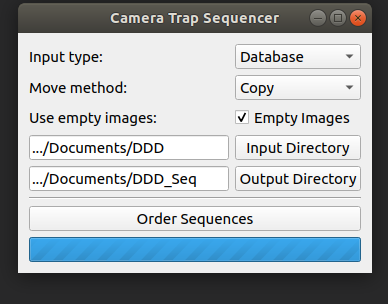
\includegraphics[scale=0.5]{img/CameraTrapSequencer.png}
	\caption{Der Camera Trap Sequencer im Linux-Design.}
\end{figure}

\subsection{Camera Trap Sequencer}

Der Camera Trap Sequencer ermöglicht es dem Anwender seine Datenbank mit Kamerafallenbildern unkompliziert und schnell auf Sequenzen aufzuteilen. Als Eingabe kann sowohl eine komplette Datenbank als auch ein einzelner Ordner mit Bildern benutzt werden. Man kann sich zwischen dem Verschieben und Kopieren der Bilder entscheiden. Das Verschieben von Bildern hat den Vorteil, dass keine Daten dupliziert werden. Die ursprüngliche Ordnerstruktur bleibt momentan jedoch noch erhalten. 

Abschließend hat man im Fall einer Bilddatenbank die Möglichkeit sich dafür zu entscheiden mit Informationen über leere Bilder zu speichern. Alle vorsortierten Datenbanken haben Verzeichnisse mit dem Namen \enquote{empty}, in denen sich Bilder auf Sequenzen befinden, auf denen keine Tiere zu sehen sind. Unsere Segmentierungstechnik PCA ist darauf angewiesen möglichst auf möglichst langen Bildsequenzen angewendet zu werden. Deshalb ist es nützlich, False-Positives mitzuverwenden, insbesondere weil leere Bilder einen großen Beitrag zur Berechnung eines leeren Hintergrundbilds leisten können. Da wir als Label für die Klassifizierung aber die Namen der Tierordner benutzen, müssen diese vor der Klassifizierung aussortiert werden. Deshalb speichern wir, falls die empty-Option gesetzt ist, eine Textdatei mit den Dateipfaden aller leeren Bilder, die dann im Anschluss an PCA aussortiert werden können. \\
Der Camera Trap Sequencer selbst ist mit PyQt5 umgesetzt. Er zeichnet sich deshalb durch ein natives Design auf jeder Plattform aus.

%!TEX root = ../ausarbeitung.tex
\section{ Lokalisierung mit Principal Components Analysis (PCA)}
Die automatische Lokalisierung von Objekten in digitalen Bildern ist ein wesentlicher Bestandteil vieler Anwendungen. 
Für das Lokalisierungsproblem in dieser Arbeit bietet sich die Verwendung von der Methoden \textit{Hintergrund-Subtraktion} und \textit{Sliding-Window} mit PCA an.

\subsection{Hintergrundapproximation mit PCA}
Um Bewegungen in Bildsequenzen erkennen zu können, wird in der Praxis sehr häufig das Verfahren der \textit{Hintergrund-Subtraktion} angewandt. Dabei handelt es sich um ein klassisches Verfahren aus dem Bereich der Bilderkennung. Das Hintergrundbild kann mithilfe von PCA approximiert werden. Anschließend wird das Vordergrundbild über die Differenz zum Hintergrundbild extrahiert. PCA, oder auch Hauptkomponentenanalyse, ist ein statistisches Verfahren um große Mengen von Datensätzen zu vereinfachen und zu strukturieren, indem die Datenpunkte im $p$-dimensionalen Raum $R^p$ in einen $q$-dimensionalen Unterraum ${R} ^{q}$ mit ($q<p$) projiziert werden. Diese Transformation muss dabei so gewählt werden, dass möglichst wenig Information verloren geht. 
Grundsätzlich benutzt PCA die \textit{Niedrigrangapproximation}. Damit kann eine Matrix durch eine andere Matrix im allgemeinen Rang angenähert werden. Sei eine Matrix $A$ mit $Rang(A) = r$ und $r > k$:
\begin{equation}
\min_{rang(A)=k}||A-B||_2 
\end{equation}
Dabei soll die Differenz zwischen $A$ und $B$ minimiert werden. Mithilfe der \textit{Singulärwertzerlegung} (SVD) können die Singulärwerte einer Matrix abgelesen werden. Die SVD von Matrix $A$ ist dann:
\begin{equation}
A = U \Sigma V^T
\end{equation}
Somit kann ein Hintergrundbild aus einer Sequenz von Bildern wie folgt approximiert werden (Abbildung~\ref{fig:approx}):
\begin{itemize}
\item{Berechne Singulärwertzerlegung aller Bildern von Sequenz $X$:}
\begin{equation}
SVD(X)= C = U \Sigma V^T
\end{equation}
\item{Leite die Matrix ${\Sigma_k}$ von ${\Sigma}$ her, sodass die Werte ${n - k}$  entlang der Diagonale durch 0 ersetzt werden.}
\item{Dies ergibt die Niedrigrangapproximation von Matrix $X$:}
\begin{equation}
SVD(X)_k=C_k = U\Sigma_kV^T \quad\quad mit  \quad  \Sigma_k = diag(\sigma_1, ..., \sigma_k,0,...,0)
\end{equation}
\end{itemize}
\newpage
\begin{center}
\begin{tabular}{ccccc}
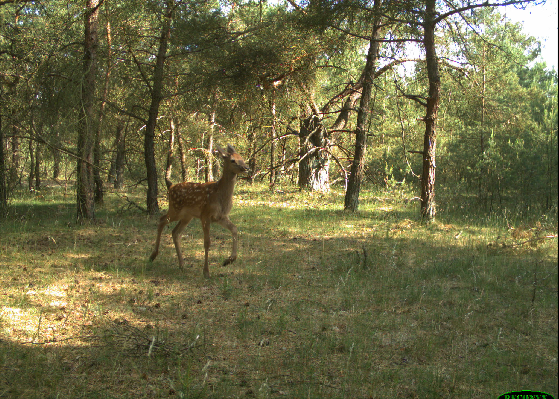
\includegraphics[width=2.3cm]{img/Segmentierung/original-image}
&
\includegraphics[width=2.3cm]{img/Segmentierung/seq2}
&
\includegraphics[width=2.3cm]{img/Segmentierung/seq4}
&
\includegraphics[width=2.3cm]{img/Segmentierung/seq3}
&
\includegraphics[width=2.3cm]{img/Segmentierung/seq5}\\
(a) & (b) &(c)&(d)&(e)
\end{tabular}
\end{center}
\begin{center}
\begin{tabular}{c}
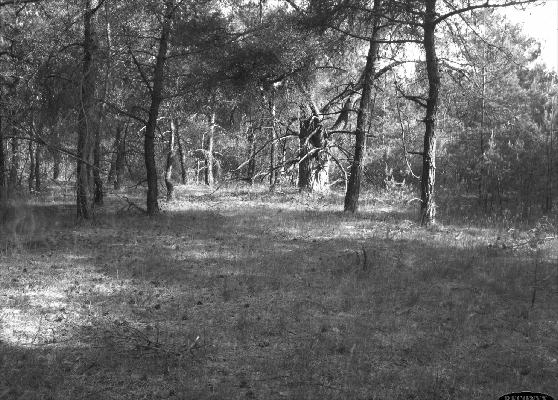
\includegraphics[width=4cm]{img/Segmentierung/background-image}\\
(f) 
\end{tabular} 
\captionof{figure}{(a)-(e) Bilder aus einer Sequenz und (f) das approximierte Hintergrundbild.}
\label{fig:approx}

\end{center}

\noindent Anschließend kann das Vordergrundbild durch die klassische \textit{Hintergrund-Subtraktion} extrahiert werden (Abbildung~\ref{fig:foreground}).

\begin{center}
\begin{tabular}{c}
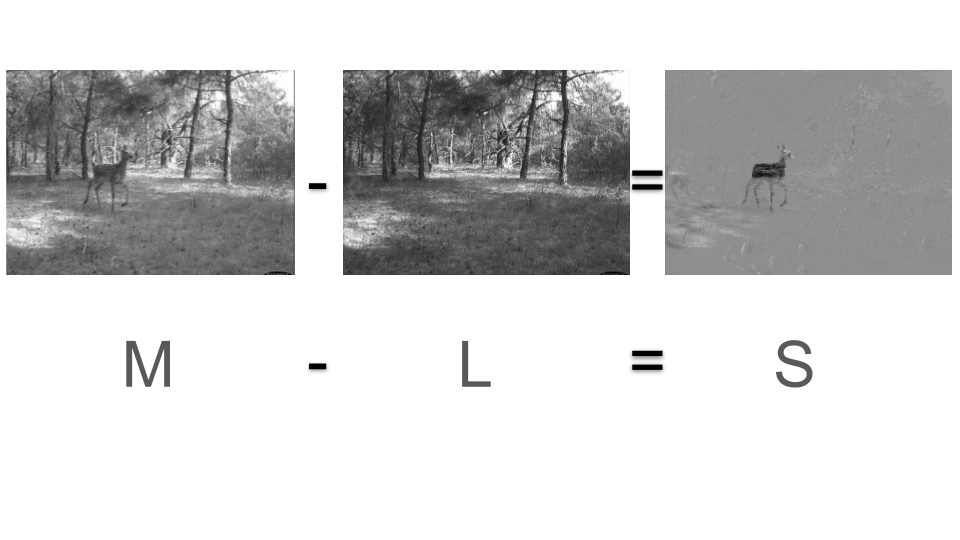
\includegraphics[width=6cm]{img/Segmentierung/foreground-image}
\end{tabular}
\captionof{figure}{Das Vordergrundbild ergibt sich durch die Subtraktion des approximierten Hintergrundbildes.}
\label{fig:foreground}
\end{center}
\noindent Zum Nachbearbeitung des Vordergrundes gehört eine Vielzahl von Operationen 
z.B. \textit{morphologische Operationen, Thresholding} und \textit{Filterung}.
Damit können kleinere Bildstrukturen und Rauschen entfernt, vergrößert, geschlossen oder aufgefüllt werden. Können jedoch diese Operationen zu einer Veränderung der Größe der Vordergrundelemente führen, was zur Lokalisierung des Elements aber keinen Störfaktor ergibt. Durch Kombination der Operationen in einer bestimmten Reihenfolge kann Größenveränderung verhindert und dennoch die Vorteile der Operationen genutzt werden. Durch \textit{Opening} werden zunächst kleine Strukturen bzw. Rauschen, welches zum Hintergrund gehört, entfernt. Danach werden kleine Löcher innerhalb der Vordergrundelemente durch \textit{Closing} geschlossen. In (Abbildung~\ref{fig:pipe}) ist eine Kombination dieser  Pipeline zur Nachbearbeitung des Vordergrundes benutzt worden.
\begin{center}
\begin{tabular}{c}
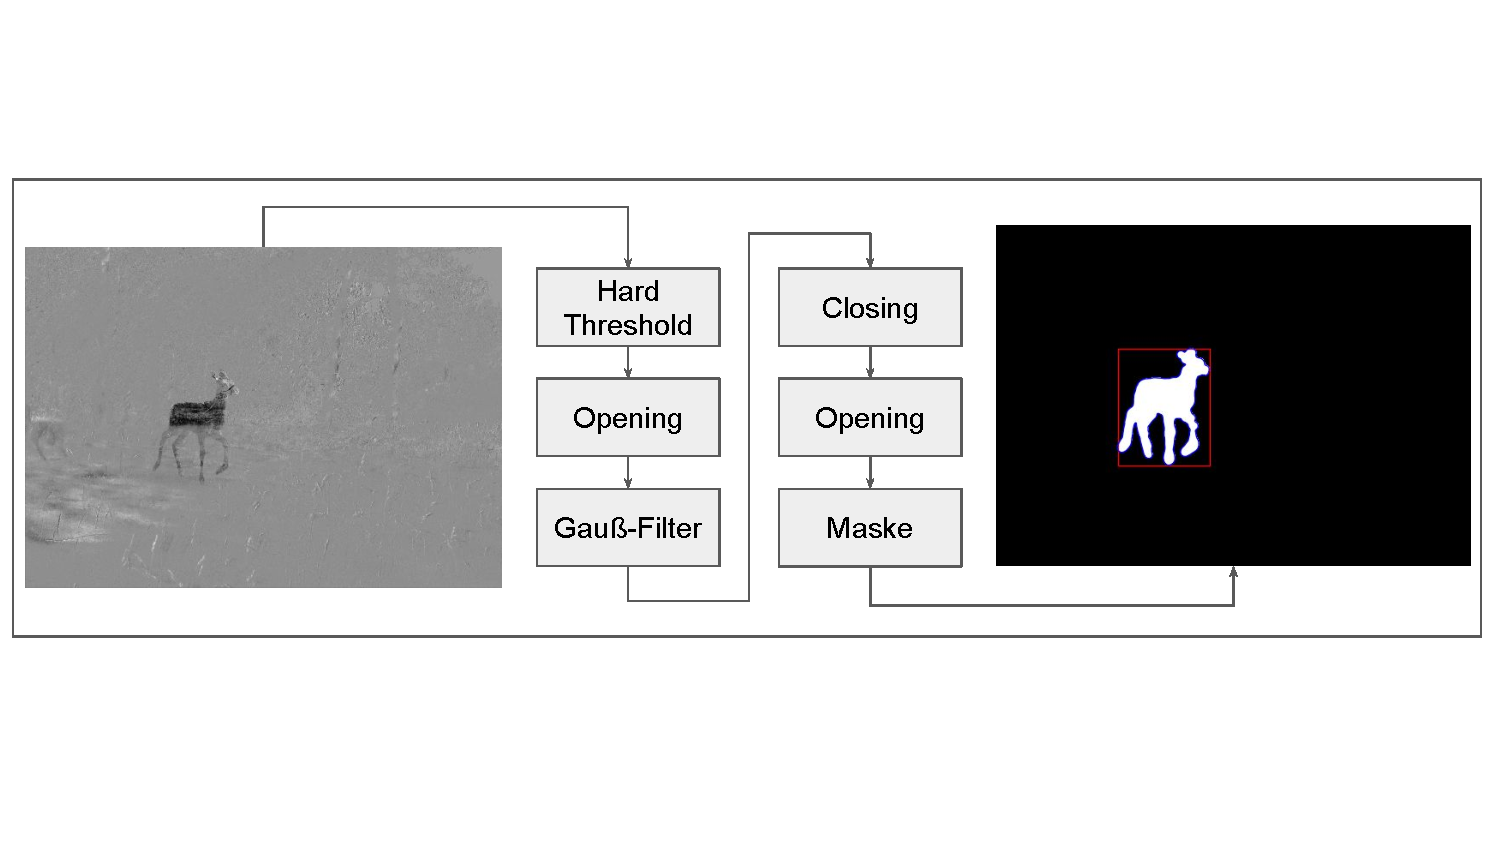
\includegraphics[trim={0 3cm 0cm 3cm},clip=true,width=13cm]{img/Segmentierung/pipe.pdf}
\end{tabular}
\captionof{figure}{Die Pipeline der Nachbearbeitung des Vordergrundbildes. Durch \textit{Opening} und \textit{Closing} werden kleine Bildstrukturen bzw. Rauschen entfernt und kleine Löcher geschlossen werden. Die Gauß-Filterung dient in diesem Fall dazu, die Silhouette des Vordergrundelements grob zu vergrößern.}
\label{fig:pipe}
\end{center}
\subsection{Sliding-Window Lokalisierung mit PCA}
Sliding-Window ist eine Brute-Force-Suche über das Bild mit fester Fenstergröße, um Objekte zu finden. Für jedes dieser Fenster wird ein Bildklassifikator angewendet, um zu bestimmen, ob das Fenster ein bekanntes Objekt enthält. In diesem Fall wird PCA als Objekt-Klassifikator angewandt.
\subsection{Objektdetektion mit PCA}
Jedes Bild ist ein Punkt in einem hochdimensionalen Raum. Durch das PCA-Verfahren lassen sich die Datenpunkte in einen niederdimensionalen Unterraum abbilden. PCA sucht die ersten $k$-Hauptkomponenten, welche die Daten mit einer maximalen Varianz beschreiben. Damit wird es eine niederdimensionale Darstellung gefunden, bei der die Klassifizierung leichter wird.\\

\subsubsection{Algorithmus}
\begin{itemize}
\item{Phase I: Initialisierung}
\begin{itemize}
\item{Berechne das Mittelwertbild der Trainingsbilder}
\begin{equation}
\mu = \frac{1}{n}\sum^n_{i=1}{x_i} 
\end{equation}
\item{Berechne die zentrierten Daten durch Subtraktion der Trainingsbilder vom Mittelwertbild}
\begin{equation}
C = X - \mu
\end{equation}
\item{Berechne die Eigenwerte und Eigenvektoren für die Kovarianzmatrix $CC$$^T$}

\begin{equation}
\mathbf{SVD}(C) =\mathbf{U} \Sigma V^T 
\end{equation}
\item{Projiziere die Trainingsbilder in den $r$-Unterraum}
\begin{equation}
\mathbf{Y}=\mathbf{U}^{T}_{r}C
\end{equation}
\end{itemize}
\item{Phase II: Klassifikation}\\
Gegeben ist ein unbekanntes Bild  $M$
\begin{itemize}
\item{Projiziere das Bild $M$ in den $r$-Unterraum}
\begin{equation}
\mathbf{W}=\mathbf{U}^{T}_{r} (M - \mu)
\end{equation}
\item{Finde den nächsten Nachbarn zwischen den projizierten Trainingsbildern $\mathbf{Y}$ und dem projizierten Bild $\mathbf{W}$}.
\end{itemize}
\end{itemize}
Die Sliding-Windows laufen das Bild mit unterschiedlichen Fenstergrößen durch. Demnach werden Schnittbilder einzelne mit PCA klassifiziert. Dabei wird der nächste Nachbar der projizierten Schnittbilder gefunden und zugeordnet (Abbildung~\ref{fig:loc}).

\begin{center}
\begin{tabular}{c}
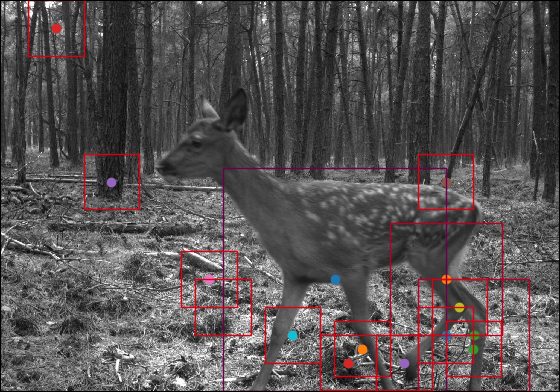
\includegraphics[width=8cm]{img/Segmentierung/localisation}
\end{tabular}
\captionof{figure}{ Lokalisierung mit Sliding-windows und PCA.}
\label{fig:loc}
\end{center}

%!TEX root = ../vortrag.tex
\section{Lokalisierung und Klassifizierung mit HOGs und SVMs}
\begin{frame}[t,fragile]{???}
	bla
\end{frame}

%!TEX root = ../vortrag.tex
\section{Klassifizierung mit Locality-constrained Linear Coding, Spatial Pyramid Matching und linearen SVMs}
\begin{frame}[t,fragile]{Übersicht}
	\begin{itemize}
		\item Ansatz zur Klassifizierung von \citet{lsp06}
		\item ursprünglich zur Klassifikation von Szenen benutzt (z.B. Gebirge, Strand, Stadt)
		\item Erweiterung des Bag-of-Words-Ansatzes, bei dem auch die räumliche Anordnung von Features im Bild beachtet wird
		\item Aufbau des Algorithmus:
		\begin{enumerate}
			\item berechne SIFT-Features über zufälligen Bildausschnitten und clustere sie in Codebook
			\item berechne für jedes Eingabebild dichte SIFT-Features in Spatial Pyramid
			\item wende Locality-constrained Linear Coding (LLC) auf jedem Feature an
			\item poole die LLC-Codes aus jedem Spatial Bin
			\item konkateniere alle gepoolten Codes der Spatial Pyramid
			\item normalisiere diese konkatenierten Codes
			\item trainiere damit eine Support Vector Machine mit linearem Kernel
		\end{enumerate}
	\end{itemize}
\end{frame}

\begin{frame}[t, fragile]{Spatial Pyramid}
	\begin{figure}
		\centering
		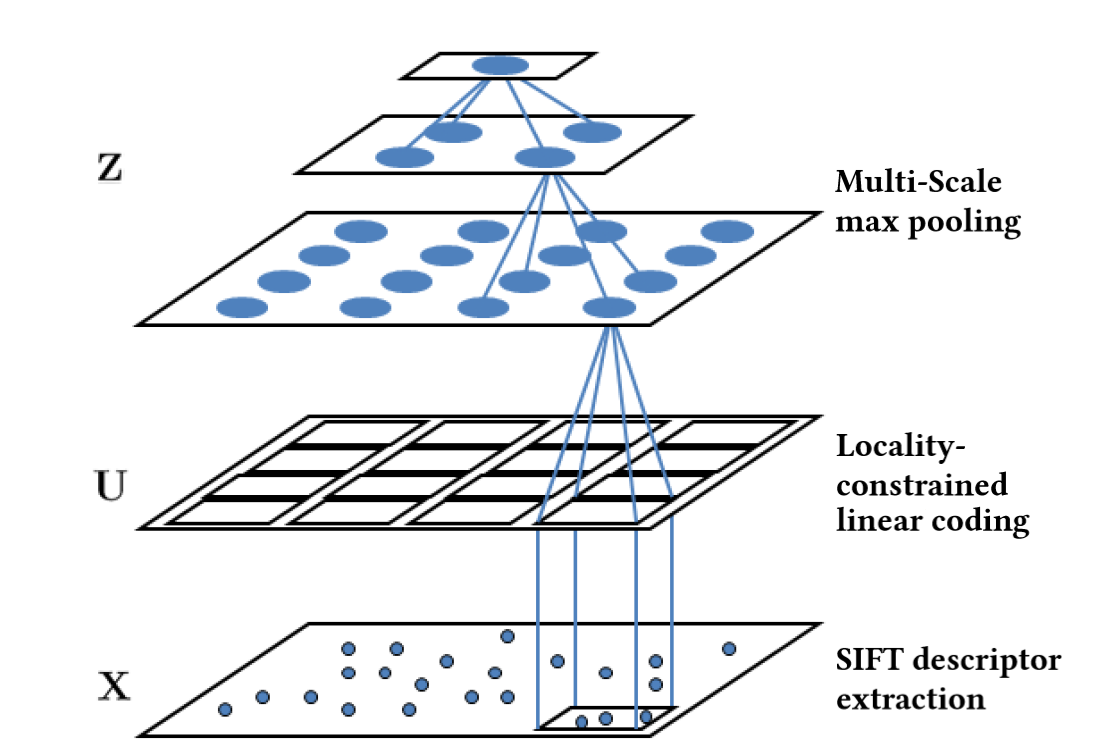
\includegraphics[scale=0.25]{img/architecture}
		\caption{Architektur des Spatial-Pyramid-Matching-Ansatzes \cite{yygh09}}
	\end{figure}
\end{frame}

\begin{frame}[t, fragile]{Locality-constrained Linear Coding (LLC)}
	\begin{figure}
		\centering
		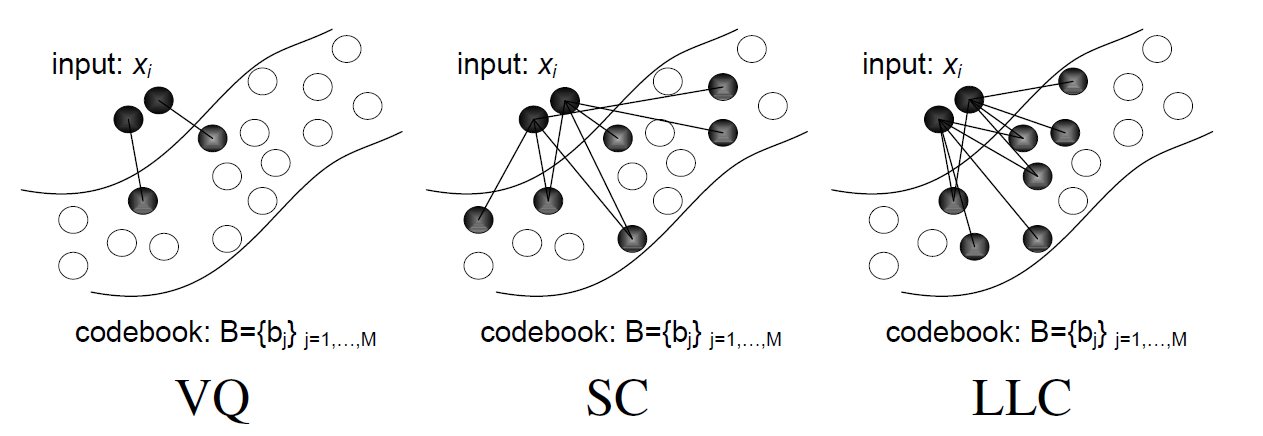
\includegraphics[scale=0.7]{img/quant_comp.png}
		\caption{Vergleich verschiedener Quantisierungsstrategien \cite{wyylhg10}}
	\end{figure}
\end{frame}

\begin{frame}[t, fragile]{Locality-constrained Linear Coding (LLC) II}
	\begin{itemize}
		\item Gegeben D-dimensionale Features $X = [x_1, \dots, x_N] \in \mathbb{R}^{(D \times N)}$ und Codebook mit M Einträgen $B = [b_1, \dots, b_M] \in \mathbb{R}^{(D \times M)}$. 
		\item Gesucht: lokale Zuordnung $C = [c_1, \dots, c_N] \in \mathbb{R}^{(M \times N)}$, die Features aus $X$ Visual Words aus $B$ zuweist.  
	\end{itemize}	 
	\begin{equation}
		\min_C \sum_{i=1}^{N} ||x_i - B\cdot c_i||^2 + \lambda\cdot ||d_i \odot c_i||^2, \text{ s.t. } 1^Tc_i = 1 \forall i
	\end{equation}
	\begin{itemize}
		\item Hierbei ist $\odot$ die elementweise Multiplikation und $d_i$ ist ein Distanzterm, der die Ähnlichkeit von Feature $x_i$ zu allen Visual Words des Codebooks wiederspiegelt.
	\end{itemize}
	\begin{equation}
		d_i = \exp \left( \frac{ \mathop{dist}(x_i, B)}{\sigma} \right)
	\end{equation}
\end{frame}

\begin{frame}[t, fragile]{Analytische Lösung von LLC}
	\begin{itemize}
		\item Anders als viele andere Quantisierungsstrategien lässt sich LLC analytisch lösen.
		\begin{itemize}
			\item wir können selber etwas programmieren
			\item (angeblich) in der Praxis schneller
		\end{itemize}
	\end{itemize}
	\begin{equation*}
		\text{ber. Kovarianzmatrix } C_i = (B-1x_i^T)(B-1x_i^T)^T
	\end{equation*}
	\begin{equation}
		\text{Löse LGS: } (C_i + \lambda\mathop{diag}(d_i)) \cdot \tilde{c}_i = (1, \dots, 1)^T
	\end{equation}
	\begin{equation}
	\text{Normalisiere: } c_i = \frac{\tilde{c}_i}{1^T\tilde{c}}
	\end{equation}
\end{frame}

\begin{frame}[t, fragile]{Pooling und Normalisierung}
	\begin{itemize}
		\item poole die LLC-Codes für jeden Spatial Bin:
		\begin{itemize}
			\item sum pooling: $c_{out} = c_1 + \dots + c_N$
			\item max pooling: $c_{out} = \max(c_1, \dots, c_N)$
		\end{itemize}
		\item konkateniere die gepoolten LLC-Codes für jeden Spatial Bin:
		\begin{itemize}
			\item insgesamt 21 konkatenierte LLC-Codes (Level 0: 1, Level 1: 4, Level 2: 16)
		\end{itemize}
		\item normalisiere die konkatenierten Codes:
		\begin{itemize}
			\item sum normalization: $c_{out} = c_{in} / \sum_{j}c_{in}(j)$
			\item $\mathit{l}^2$ normalization: $c_{out} = c_{in} / ||c_{in}||_2$
		\end{itemize}
		\item in der Praxis haben sich Max-Pooling und $\mathit{l}^2$-Normalisierung durchgesetzt \cite{wyylhg10}
	\end{itemize}
\end{frame}

\begin{frame}[t, fragile]{Support Vector Machine mit linearem Kernel}
	\begin{itemize}
		\item Empirische Tests haben ergeben, dass Spatial-Pyramid-Matching-Codes gut linear separierbar sind und diese bessere Ergebnisse liefern als nicht-lineare Kernel \cite{lsp06}.
		\item Benutze Support Vector Machine mit linearem Kernel $k(z_i, z_j) = z_i^Tz_j$ und \emph{quadratic hinge loss}-Funktion.
		\begin{itemize}
			\item Training in $\oh(N)$ und Testen in $\oh(1)$ statt $\oh(N^3)$ und $\oh(N)$ für nicht-lineare Mercer-Kernel.
		\end{itemize}
	\end{itemize}
\end{frame}

\begin{frame}[t, fragile]{Umsetzung}
	\begin{itemize}
		\item Programmiersprache Python
		\item größtenteils mit \emph{numpy} umgesetzt
		\item Parallelisierung der Enkodierung von Level 2 Spatial Bins mit Pythons Multiprocessing
		\item Berechnung der SIFT-Features mit OpenCV
		\item Clustering für Codebook mit Scikit-learns \emph{MiniBatchKMeans} \cite{sklearn}
		\begin{itemize}
			\item deutlich schnellere Laufzeit als \emph{KMeans}
			\item identische Ergebnisse
		\end{itemize}
		\item Scikit-Learns \emph{LinearSVC} als Support Vector Machine \cite{sklearn}
		\begin{itemize}
			\item setzt linearen Kernel und quadratische Hinge-Loss-Funktion schon um
			\item effizienter als SVC(kernel='linear')
		\end{itemize}
	\end{itemize}
\end{frame}
%!TEX root = ../ausarbeitung.tex
\newpage
\section{Evaluierung}

%!TEX root = ../vortrag.tex
\section{Ausblick}
\begin{frame}[t,fragile]{Ausblick}
	\begin{itemize}
		\item PCA funktioniert nur auf Sequenzen von Bildern
		\begin{itemize}
			\item Idee: baue während PCA Index von Bildern aller Kameras (nach Seriennummer) auf
			\item benutze diesen Index zur Segmentierung von Einzelbildern, indem diese zur Sequenz vervollständigt werden
		\end{itemize}
		\item Spatial Pyramid Matching ist momentan sehr langsam
		\begin{itemize}
			\item Bottleneck: die Berechnung der LLC-Codes, insbesondere die Lösung des linearen Gleichungssystems
			\item optimiere Code mit \emph{numba} und parallelisiere weiter \cite{numba}
		\end{itemize}
		\item Kombiniere SPM mit LLC durch verschiedene Arten von Features, wie von \cite{ywkjwh13} vorgeschlagen
		\begin{itemize}
			\item berechne Textur- oder Farbfeatures, wie beispielsweise cLBP auf dichtem Gitter
			\item Kombination mit SIFT-Features über \emph{Boosting} oder Scikit-learns \emph{Voting Classifier}
		\end{itemize} 
	\end{itemize}
\end{frame}

\nocite{*}
\section*{Quellen}
\begin{frame}[allowframebreaks,t]{\secname}
	\printbibliography
\end{frame}


\end{document}
